\section{1174031 - Muhammad Tomy Nur Maulidy}
\subsection{Memperkenalkan pemrograman paralel Python}
	Python menyediakan banyak pustaka dan kerangka kerja yang memfasilitasi kinerja tinggi
perhitungan. Namun, melakukan pemrograman paralel dengan Python bisa sangat berbahaya
karena Global Interpreter Lock (GIL).
Bahkan, interpreter Python yang paling luas dan banyak digunakan, CPython, dikembangkan di
bahasa pemrograman C. Penerjemah CPython membutuhkan GIL untuk keamanan thread
operasi. Penggunaan GIL menyiratkan bahwa Anda akan menemukan kunci global ketika Anda mencoba
untuk mengakses objek Python yang ada di dalam utas. Dan hanya satu utas dalam satu waktu yang bisa
memperoleh kunci untuk objek Python atau API C.
Untungnya, masalahnya tidak terlalu serius, karena, di luar ranah GIL, kita bisa leluasa menggunakannya
paralelisme. Kategori ini mencakup semua topik yang akan kita bahas dalam bab-bab berikutnya,
termasuk multiprocessing, komputasi terdistribusi, dan komputasi GPU.
Jadi, Python tidak benar-benar multithreaded. Tapi apa itu utas? Apa itu proses? Dalam
bagian berikut, kami akan memperkenalkan dua konsep dasar ini dan bagaimana mereka
ditangani oleh bahasa pemrograman Python.
\subsection{Proses dan utas}
Utas dapat dibandingkan dengan proses yang ringan, dalam arti bahwa mereka menawarkan manfaat yang serupa untuk proses, tanpa, bagaimanapun, membutuhkan teknik komunikasi yang khas proses. Utilitas ini memungkinkan Anda untuk membagi aliran kontrol utama dari suatu program menjadi beberapa secara bersamaan menjalankan aliran kontrol. Sebagai gantinya, proses memiliki ruang pengalamatan sendiri dan sumber daya mereka sendiri. Kemudian komunikasi antar bagian kode berjalan Proses yang berbeda hanya dapat terjadi melalui mekanisme manajemen yang tepat, termasuk pipa, kode FIFO, kotak surat, area memori bersama, dan menyampaikan pesan. Utas, di sisi lain, memungkinkan pembuatan bagian bersamaan dari program, di mana setiap bagian dapat mengakses ruang alamat, variabel, dan konstanta yang sama.
\subsection{Praktek}
\begin{enumerate}
	\item do something
    \lstinputlisting[firstline=8, lastline=12]{src/kelompok1/do_something.py}
	\hfill\break
	\item serial test
	\hfill\break
	\lstinputlisting[firstline=8, lastline=22]{src/kelompok1/serial_test.py}
	\item multithreading test
	\hfill\break
	\lstinputlisting[firstline=8, lastline=30]{src/kelompok1/multithreading_test.py}
	\item multiprocessing test
	\hfill\break
	\lstinputlisting[firstline=8, lastline=30]{src/kelompok1/multiprocessing_testpy.py}
\end{enumerate}
\subsection{Percobaan}
\begin{enumerate}
	\item Menjalankan Serial Test
	\begin{figure}[H]
		
\includegraphics[width=4cm]{figures/kelompok1/1/tomy/test1.PNG}
		\centering
		\caption{Menjalankan Serial Test}
	\end{figure}
	\begin{figure}[H]
		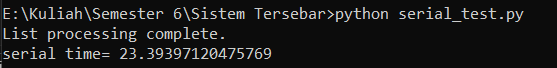
\includegraphics[width=4cm]{figures/kelompok1/1/tomy/hasil1.PNG}
		\centering
		\caption{Hasil Serial Test}
	\end{figure}
    \item Menjalankan Multithreading Test
	\begin{figure}[H]
		
\includegraphics[width=4cm]{figures/kelompok1/1/tomy/test2.PNG}
		\centering
		\caption{Menjalankan Multithreading Test}
	\end{figure}
	\begin{figure}[H]
		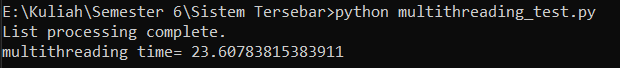
\includegraphics[width=4cm]{figures/kelompok1/1/tomy/hasil2.PNG}
		\centering
		\caption{Hasil Multithreading Test}
	\end{figure}
    \item Menjalankan Multiprocessing Test
	\begin{figure}[H]
		
\includegraphics[width=4cm]{figures/kelompok1/1/tomy/test3.PNG}
		\centering
		\caption{Menjalankan Multiprocessing Test}
	\end{figure}
	\begin{figure}[H]
		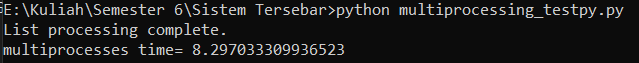
\includegraphics[width=4cm]{figures/kelompok1/1/tomy/hasil3.PNG}
		\centering
		\caption{Hasil Multiprocessing Test}
	\end{figure}
\end{enumerate}
\subsection{Bukti Tidak Plagiat}
\begin{figure}[H]
	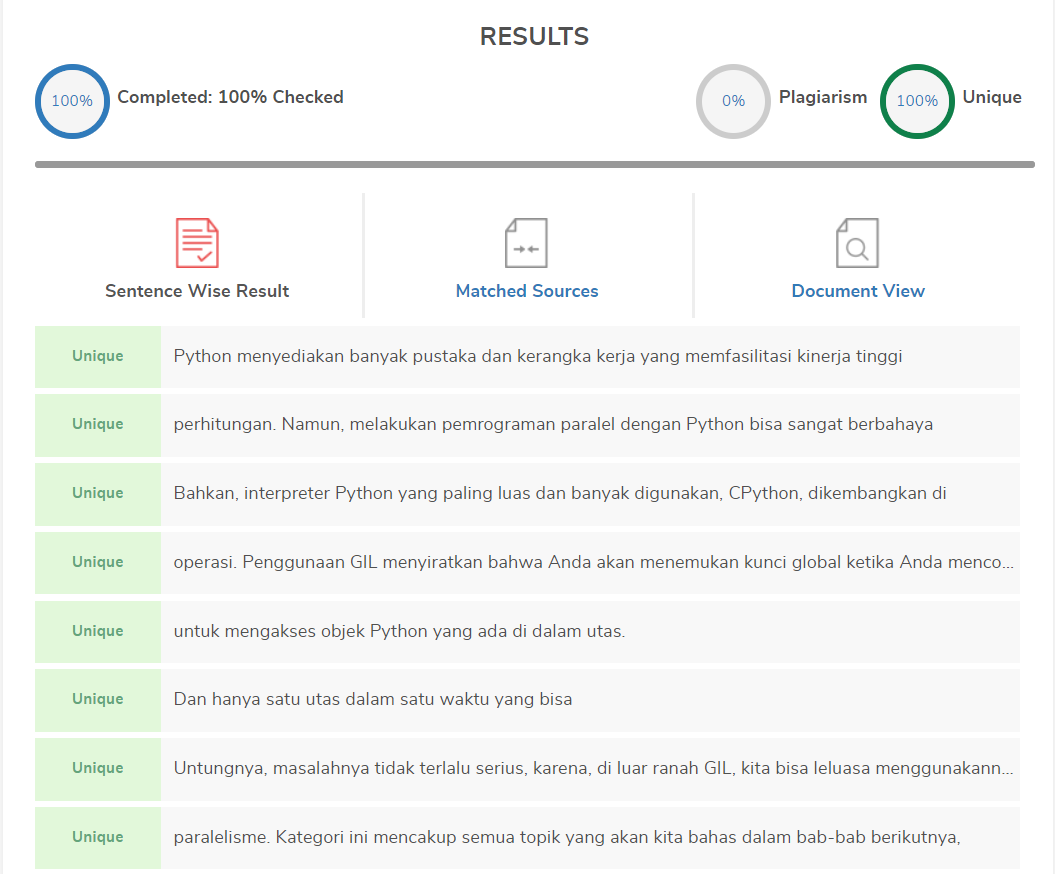
\includegraphics[width=4cm]{figures/kelompok1/1/tomy/plagiat_tomy_1.PNG}
	\centering
	\caption{Bukti Tidak Melakukan Plagiat 1}
    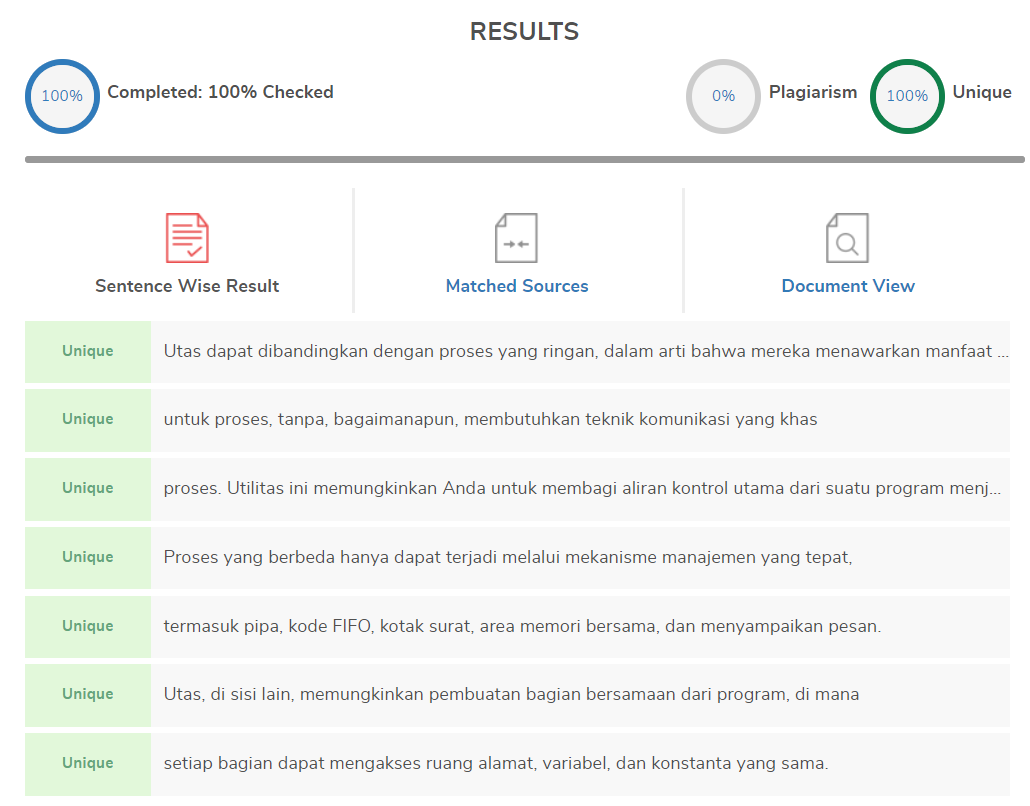
\includegraphics[width=4cm]{figures/kelompok1/1/tomy/plagiat_tomy_2.PNG}
	\centering
	\caption{Bukti Tidak Melakukan Plagiat 2}
\end{figure}